\section{Primera Pagina en Symfony}
Crear una nueva página, ya sea una página HTML o JSON, es un proceso de dos pasos:
\begin{itemize}
  \item \textbf{Crear una ruta:} Una ruta es la URL (por ejemplo, /about) a su página y apunta a un controlador
  \item \textbf{Crear un controlador}: Un controlador es un script PHP de funciones que se encargará de construir las páginas. Toma la información de respuesta creando un objeto de Symfony de tipo Response, cada uno puede contener contenido HTML, cadenas JSON o incluso archivos binarios, tanto imágenes como PDF.
\end{itemize}
\subsection{Creando una página: Route y Controller}
Supongamos que queremos crear la página - \texttt{/lucky/number} - que genera números de la suerte (de forma aleatoria) y los imprime. Para hacer eso, creamos una “Controller class” que la llamaremos LuckyController y un método “controller” que será ejecutado cada vez que vayamos a \texttt{/lucky/number}:


\begin{figure}[ht]
  \centering
  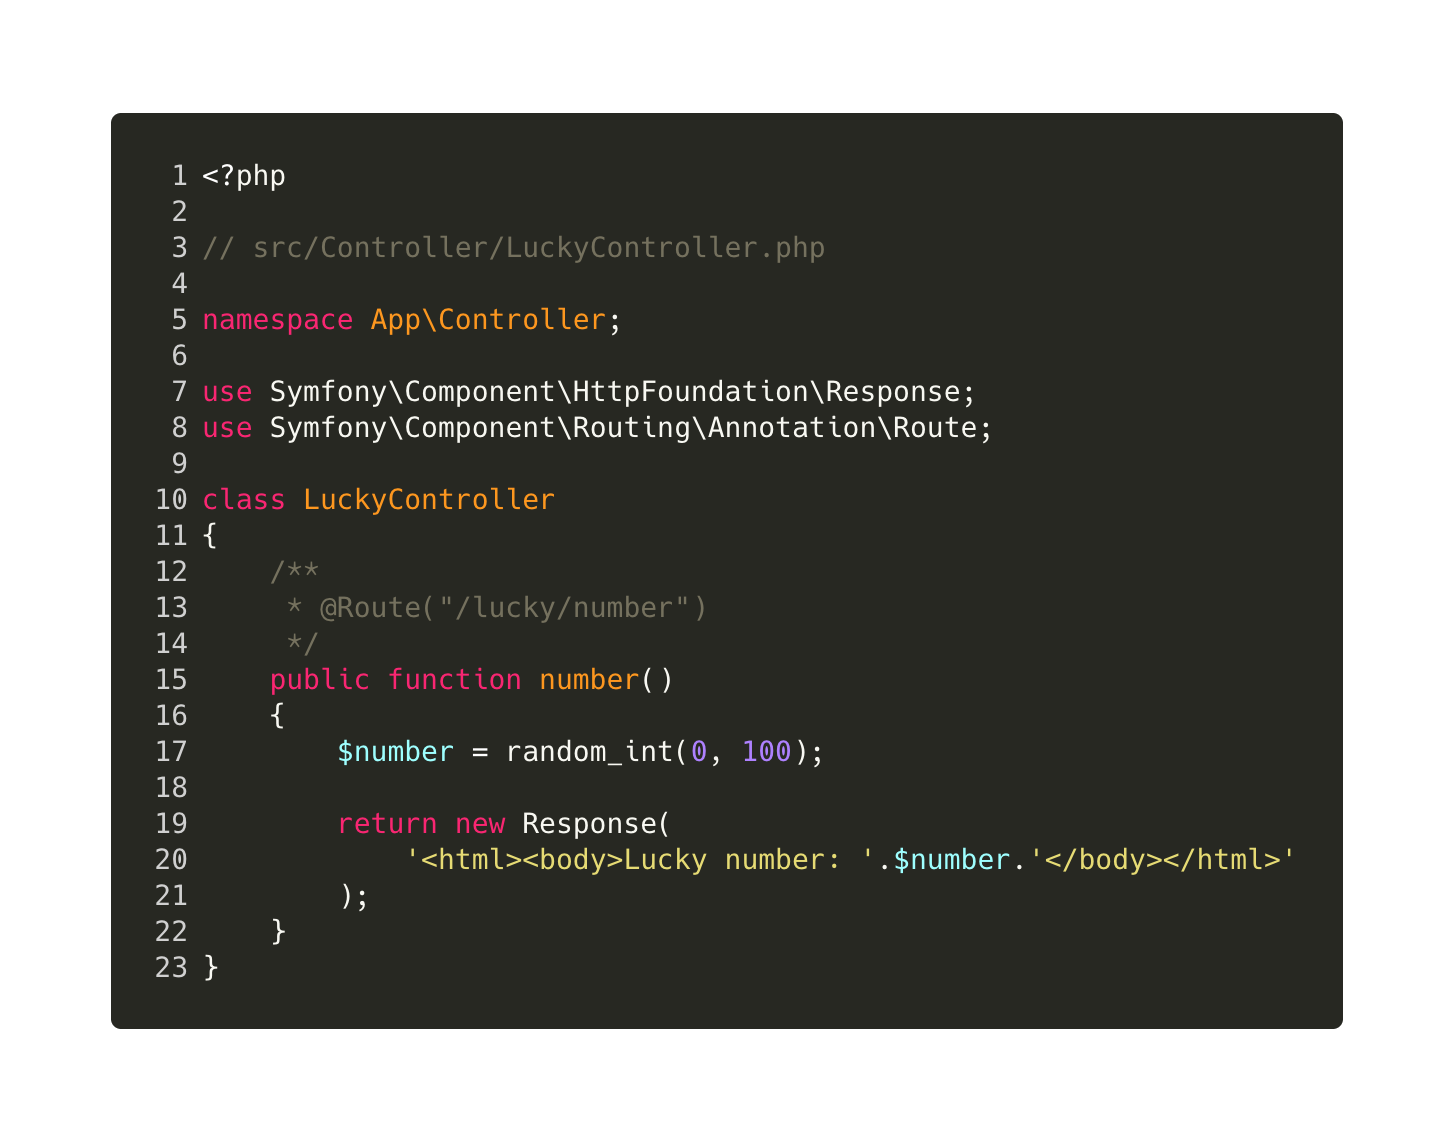
\includegraphics[width=\textwidth]{../assets/lucky_controller.png}
  \caption{Controlador \textbf{/luck/number}}
  \label{fig:lucky_controller}
\end{figure}

Podemos visualizar el resultado en \href{http://localhost:8888/lucky/number}{http://localhost:8888/lucky/number}

\begin{figure}[ht]
  \centering
  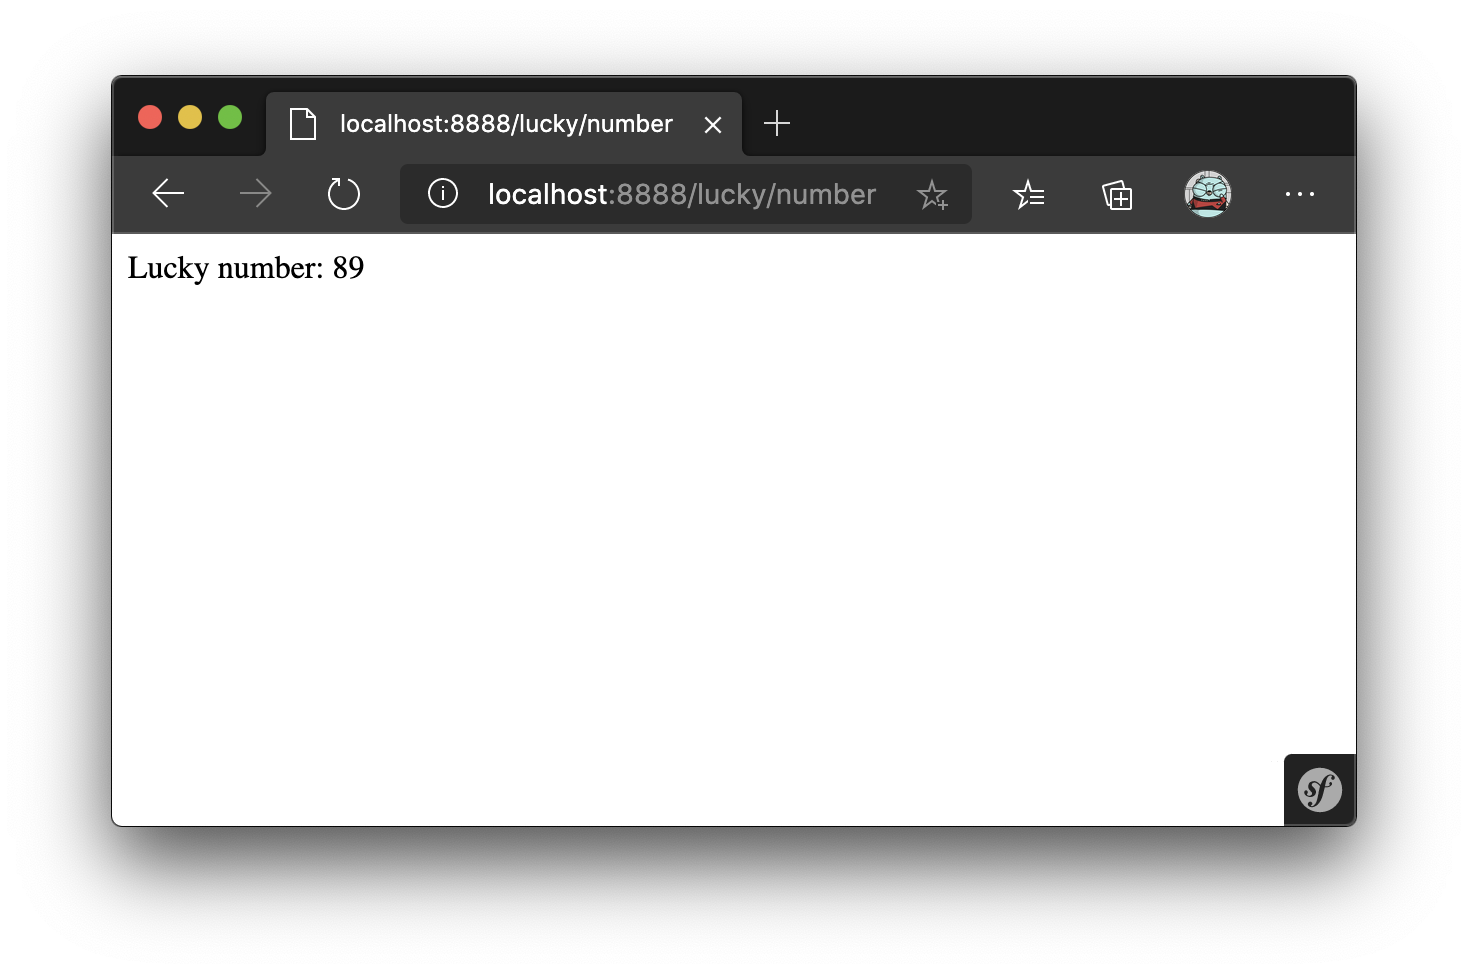
\includegraphics[width=\textwidth]{../assets/lucky_number.png}
  \caption{Respuesta \textbf{/luck/number}}
  \label{fig:lucky_number}
\end{figure}
\clearpage
\subsection{La barra de herramientas de depuración web}
Una de las características principales de Symfony es la Barra de herramientas de depuración web: una barra que muestra una gran cantidad de información de depuración en la parte inferior de la página durante el desarrollo. Todo esto está incluido de por defecti usando un paquete de Symfony llamado \texttt{symfony/profiler-pack}.

\begin{figure}[ht]
  \centering
  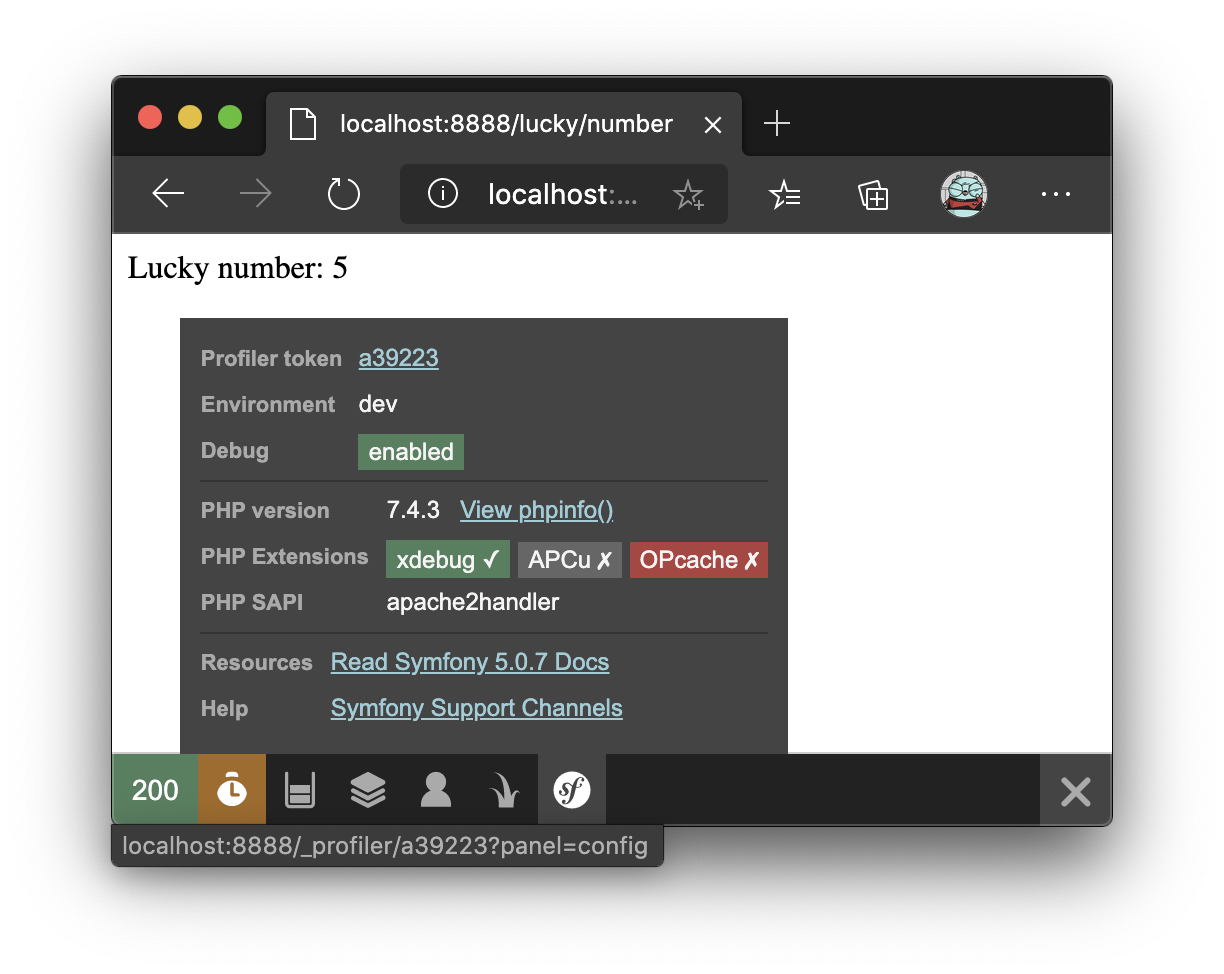
\includegraphics[width=\textwidth]{../assets/symfony_debug_bar.png}
  \caption{Barra de herramientas de depuración}
  \label{fig:symfony_debug_bar}
\end{figure}
\clearpage
\subsection{Renderizando una plantilla}

Si está devolviendo HTML desde su controlador, probablemente quiera renderizar una plantilla. Afortunadamente, Symfony viene con \href{https://twig.symfony.com/}{Twig}: un lenguaje de plantillas que es fácil, poderoso y realmente bastante divertido.
\medskip\\
Asegúrese de que LuckyController extienda la clase abstracta AbstractController de Symfony:

\begin{figure}[ht]
  \centering
  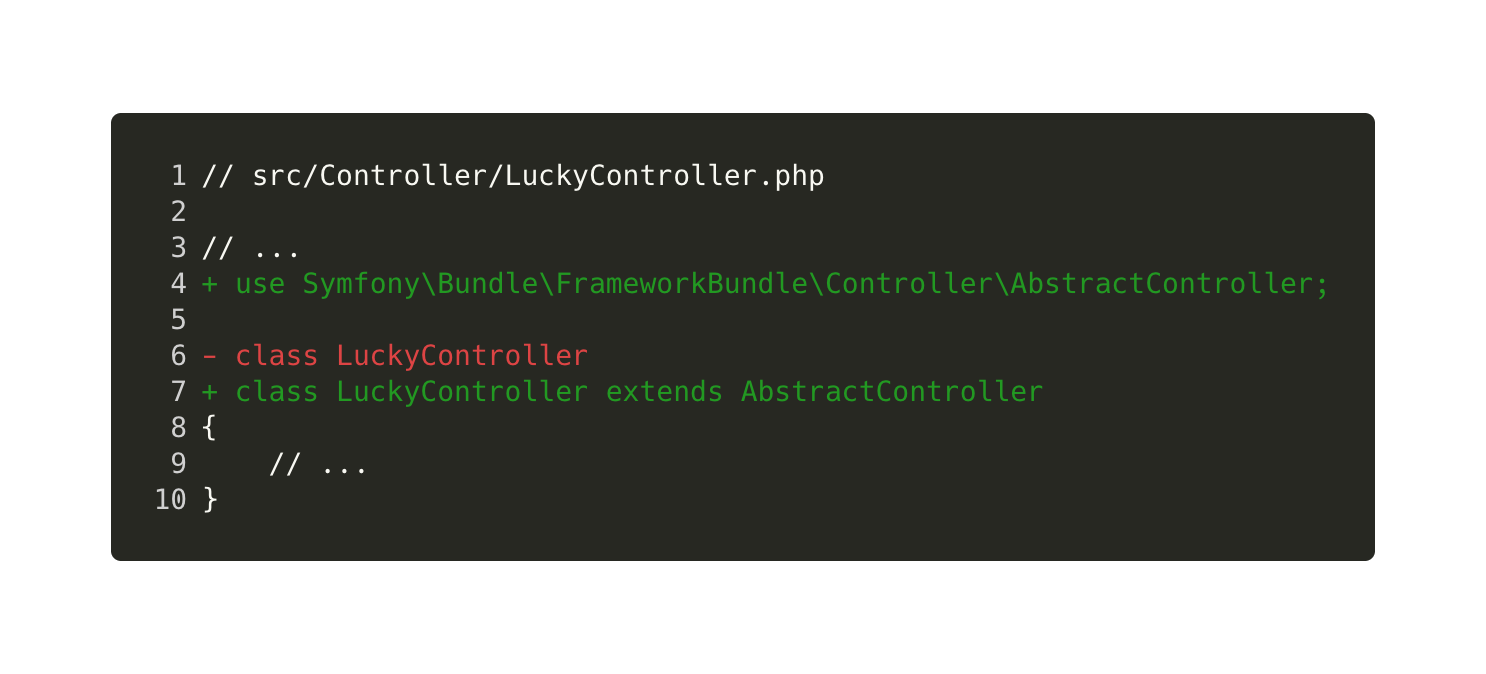
\includegraphics[width=\textwidth]{../assets/diff_lucky_controller.png}
  \caption{Heredar desde AbstractController}
  \label{fig:diff_lucky_controller}
\end{figure}

Ahora, use la práctica función \texttt{render()} para renderizar una plantilla. Pase una variable numérica para que puedas usarlo en Twig:

\begin{figure}[ht]
  \centering
  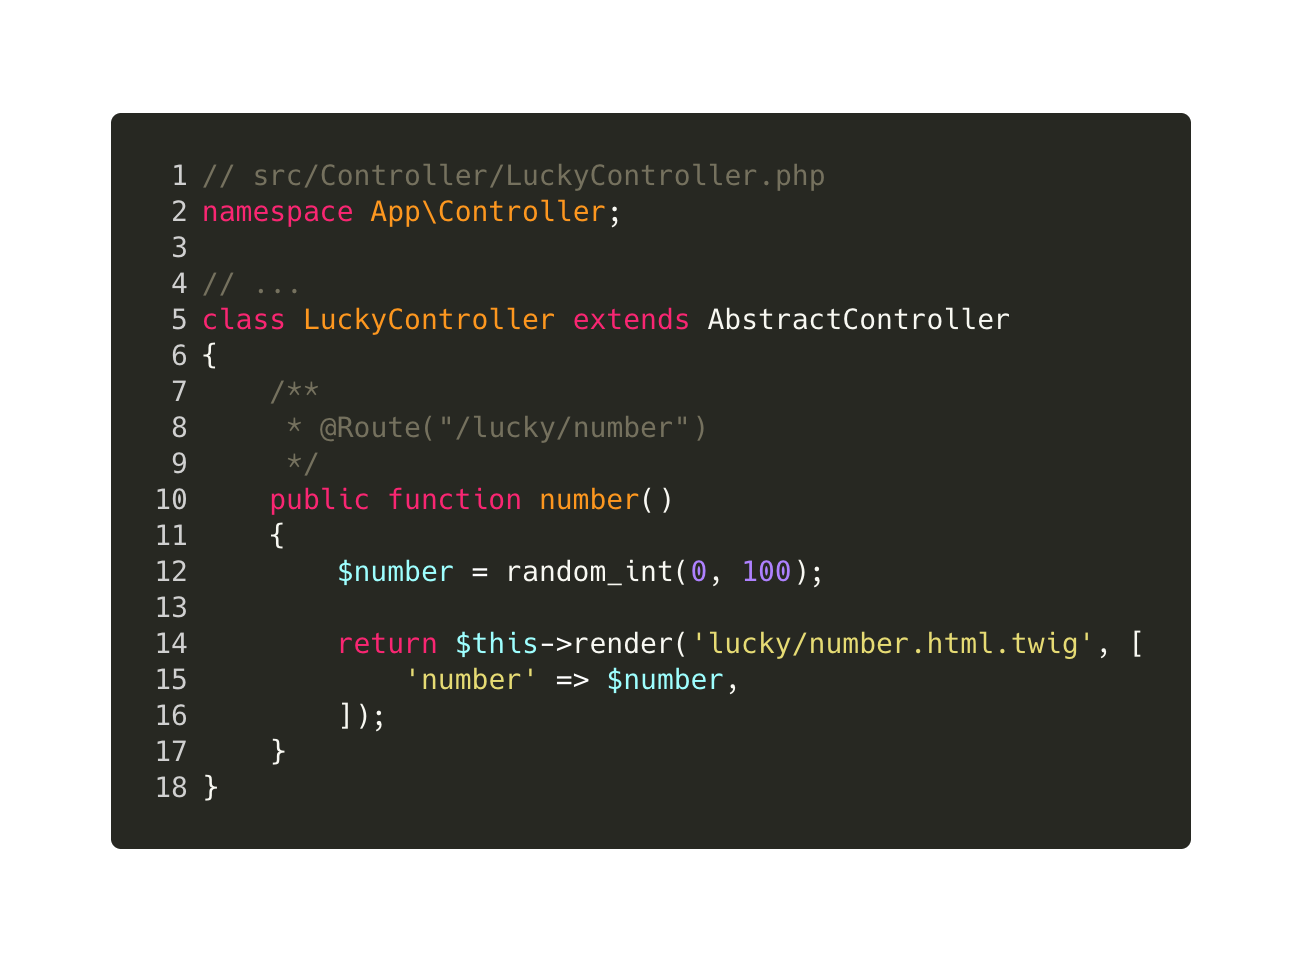
\includegraphics[width=\textwidth]{../assets/lucky_number_twig.png}
  \caption{Uso del metodo \texttt{render()}}
  \label{fig:lucky_number_twig}
\end{figure}
\clearpage
Los archivos de plantilla viven en el directorio \texttt{templates/}, que se creó automáticamente cuando instaló Twig. Cree un nuevo directorio \texttt{templates/lucky} con un nuevo archivo \texttt{number.html.twig} dentro:

\begin{figure}[ht]
  \centering
  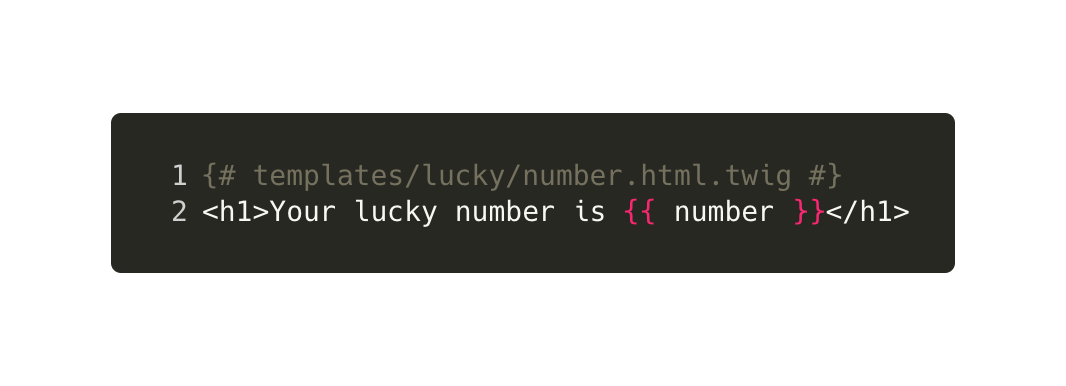
\includegraphics[width=\textwidth]{../assets/lucky_number_template.png}
  \caption{Plantilla \texttt{/lucky/number}}
  \label{fig:lucky_number_template}
\end{figure}

La sintaxis utilizada {{ number }} es para imprimir las variables en el sistema de trabajo de Twig.

\subsection{Estructura del proyecto}
Ya hemos estado trabajando en dos de las carpetas más importantes de nuestro proyecto, ahora veremos la importancia y uso de las demás dentro de la estructura que nos ofrece Symfony:
\begin{itemize}
  \item[\textbf{\texttt{config/}}] Contiene la configuración donse se configurarán rutas, servicios y paquetes.
  \item[\textbf{\texttt{src/}}] El código PHP a utilizar lo colocamos dentro de esta carpeta.
  \item[\textbf{\texttt{templates/}}] Todas las plantillas Twig viven aquí.
  \item[\textbf{\texttt{bin/}}] Aquí vive el famoso archivo \texttt{bin/console} (y otros archivos ejecutables menos importantes).
  \item[\textbf{\texttt{var/}}] Aquí es donde se almacenan los archivos creados automáticamente, como los archivos de caché (\texttt{var/cache/}) y los registros (\texttt{var/log/}).
  \item[\textbf{\texttt{vendor/}}] ¡Aquí viven bibliotecas de terceros! Estos se descargan a través del administrador de paquetes \href{https://getcomposer.org/}{Composer}.
  \item[\textbf{\texttt{public/}}] Carpeta raíz del proyecto, en esta carpeta introduciremos todos los elementos públicos(CSS, JS, imágenes...)
\end{itemize}

La mayoría de las veces, trabajaremos en \texttt{src/}, \texttt{templates/} o \texttt{config/}.